
\section{Module Integrated Conveter}

Usually, one MPPT is commonly used for many PV modules as shown in figure \ref{fig:PVsystemblocks}. This approach may lead to suboptimal efficiency of the system since the uneven power generated by the PV modules might lead to a system with a local MPP in addition to a global MPP \cite{AN1521_MC}. In figure \ref{multiple_local_MPP} a system exhibiting two MPP, due to partial shading of one of the system's PV panels, is shown. In order to ensure that the system is working in the global MPP and not in the local MPP, the inverter's controller will have to perform a voltage sweep in order to find the global MPP. This voltage sweep is a higher level of complexity in the MPPT control system \cite{AN1521_MC}. In any case, the system will not be able to get the maximum power generation, as one panel is bypassed by a diode.\todo{Here is the first time we mention the bypassed diode. Maybe give a brief explanation and add a reference. Stef}
\begin{figure}[H]
	\begin{center}
		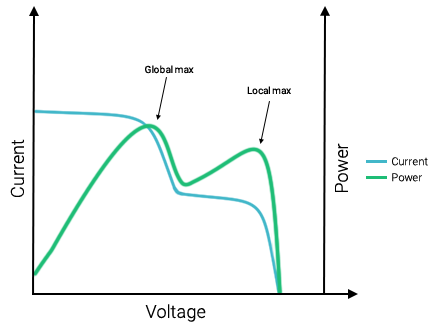
\includegraphics[width=0.65\textwidth]{../Pictures/local_MPP}
		\caption{I-V curves of a system with more than one MPP \cite{local_mpp}.}
		\label{multiple_local_MPP}
	\end{center}	
\end{figure} 
\todo{The quality of this figure isn't very good. Stef}
Another approach is using a MIC. Which is a DC to DC converter featuring a MPPT controller included in each PV module which will result in higher overall efficiencies \cite{ArchitectureMIC}. With this configuration, events like partial shading, uneven dirt, wear distribution or manufacturing imperfections are properly handled and do not affect the rest of the PV modules in the array. Also, a more detailed control of the plant is achieved since separate data from each individual panel is obtained \cite{ArchitectureMIC}. Each PV module will then be connected directly to a MIC allowing the output voltage and current to be defined by the load. This way the system is able to operate at different voltage and current levels whilst maintaining the MPP \cite{ArchitectureMIC}.

MICs can be either microinverters or DC-DC converters. In figure \ref{MIC_dcdc} a PV system using MICs is shown. Notice that $N$ panels might be used. Series or parallel connections can be used to link MICs' outputs and then connect this output to the inverter input.

\begin{figure}[H]
	\begin{center}
		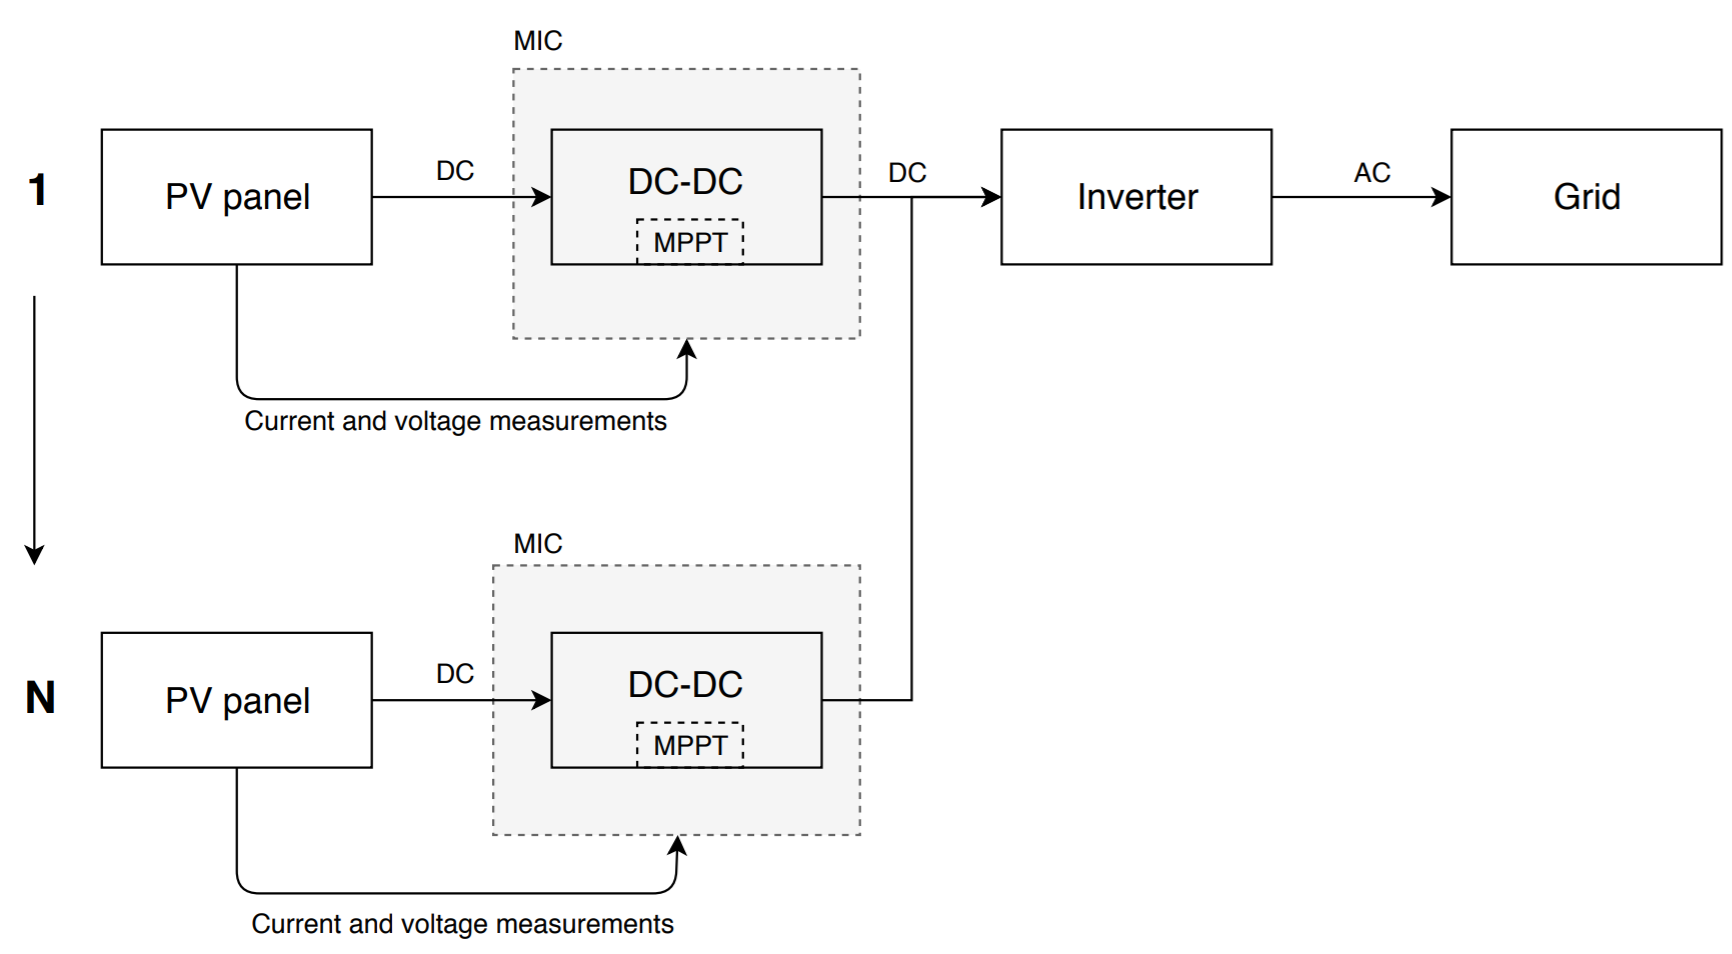
\includegraphics[width=0.8\textwidth]{../Pictures/MIC_dcdc}
		\caption{PV generation with DC-DC MIC system structure.}
		\label{MIC_dcdc}
	\end{center}	
\end{figure}

The panels with a MIC consisting on a microinverter, include a DC-DC converter with MPPT together with an inverter and are directly tied to grid. In figure \ref{microinverter_system} a microinverter system structure can be seen. For the user, this system is simpler, as only the PV must be purchase, the user does not have to worry about selecting and installing an inverter. 

\begin{figure}[H]
	\begin{center}
	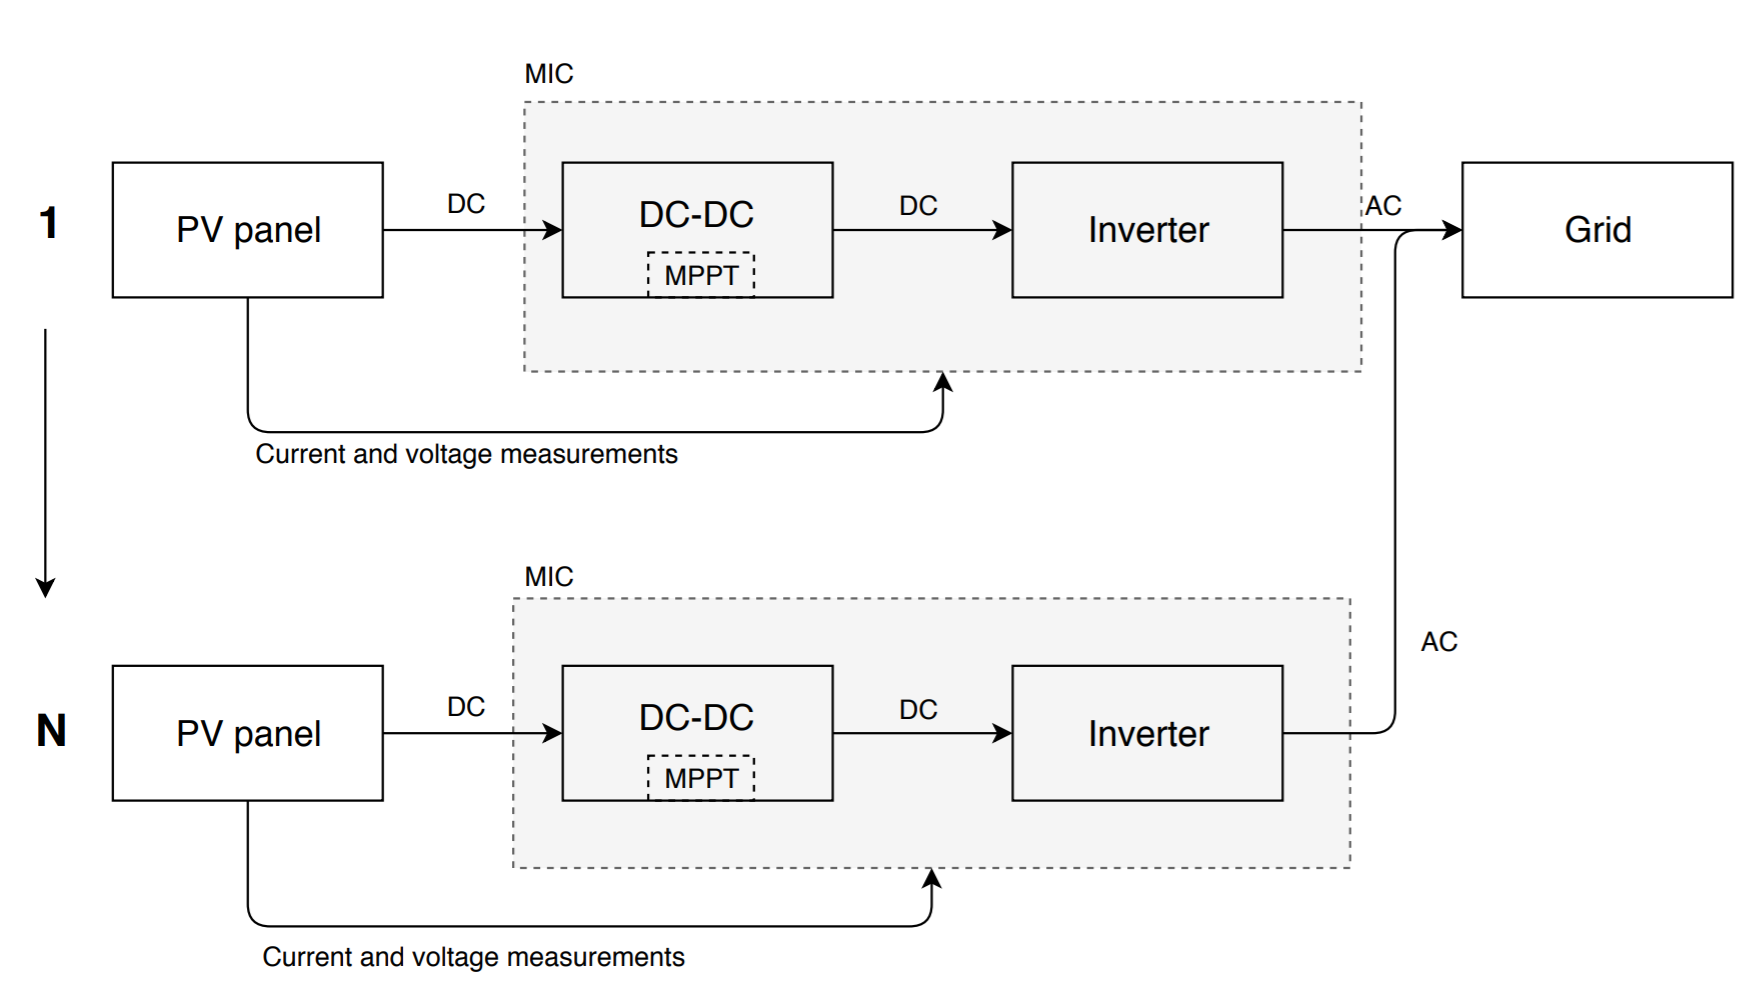
\includegraphics[width=0.8\textwidth]{../Pictures/MIC_microinverter}
		\caption{PV generation with microinverter MIC system structure.}
		\label{microinverter_system}
	\end{center}	
\end{figure}

The main advantage of the microinverter system is that it is simpler for the user, however, it implies an increase in costs and is usually less efficient than a DC-DC system with a single higher power inverter \cite{ArchitectureMIC}. Therefore, for the development of this project a DC-DC MIC will be implemented.